\documentclass[%
  a4paper,oneside,%
  %arial,
  11pt,% <10pt, 9pt>
  smallchapters,
  %style=screen,
  %sender=bottom,
  green,% <orange, green, violet>
  rgb, <cmyk>
  %mono
  ,]{tubsbook}
  
\usepackage{listings}  % for code stuff
\usepackage{xcolor}

\definecolor{codegreen}{rgb}{0,0.6,0}
\definecolor{codegray}{rgb}{0.5,0.5,0.5}
\definecolor{codepurple}{rgb}{0.58,0,0.82}
\definecolor{backcolour}{rgb}{0.95,0.95,0.92}

\lstdefinestyle{mystyle}{
	language=Python,
    backgroundcolor=\color{backcolour},   
    commentstyle=\color{codegreen},
    morekeywords={self},
    keywordstyle=\color{magenta},
    numberstyle=\tiny\color{codegray},
    stringstyle=\color{codepurple},
    basicstyle=\ttfamily\footnotesize,
    breakatwhitespace=false,         
    breaklines=true,                 
    captionpos=b,                    
    keepspaces=true,                 
    numbers=left,                    
    numbersep=5pt,                  
    showspaces=false,                
    showstringspaces=false,
    showtabs=false,                  
    tabsize=2
}


\newcommand\pythonstyle{\lstset{
	language=Python,
    backgroundcolor=\color{backcolour},   
    commentstyle=\color{codegreen},
    morekeywords={self},
    keywordstyle=\color{magenta},
    numberstyle=\tiny\color{codegray},
    stringstyle=\color{codepurple},
    basicstyle=\ttfamily\footnotesize,
    breakatwhitespace=false,         
    breaklines=true,                 
    captionpos=b,                    
    keepspaces=true,                 
    numbers=left,                    
    numbersep=5pt,                  
    showspaces=false,                
    showstringspaces=false,
    showtabs=false,                  
    tabsize=2
}}


% Python environment
\lstnewenvironment{python}[1][]
{
\pythonstyle
\lstset{#1}
}
{}




%lstset{style=mystyle}

\usepackage{bm} 
\usepackage{amsmath}
 
\renewcommand{\familydefault}{\sfdefault}
\usepackage[utf8]{inputenc}
\RequirePackage{scrlfile}
\ReplacePackage{scrpage2}{scrlayer-scrpage}

\usepackage[ngerman,english]{babel}

\usepackage{lipsum} % Blindtext-Paket
\definecolor{InAGreen}{RGB}{172,193,58}

% Titelseiten-Elemente
\title{A Statistical Approach for the Fusion of Data and
Finite Element Analysis in Vibroacoustics}
\subtitle{Untertitel}
\author{Lucas Hermann}
%\logo{Institut fuer Lorem Ipsum}
\logo{
\includegraphics{InA-Logo-rgb.pdf}}
\titleabstract{\lipsum[2]}
\titlepicture{infozentrum.jpg}
% Rückseiten-Elemente
\address{%
  Herr Mustermann\\
  Schlossallee 1\\
  33333 Darmstadt}
\backpageinfo{%
  \lipsum[5]
}
\usepackage{pdfpages}								% Einbinden von PDF-Pages
\usepackage[colorlinks,pdfpagelabels,pdfstartview = FitH,bookmarksopen = true,bookmarksnumbered = true,linkcolor = black,plainpages = false,hypertexnames = false,citecolor = black] {hyperref}
\usepackage[figure]{hypcap} 
\bibliographystyle{ieeetr}

\begin{document}

%\maketitle[image,logo=left]%[<plain/image/imagetext>,<logo=left/right>]
%\makebackpage[trisec]%[<plain/info/addressinfo>]
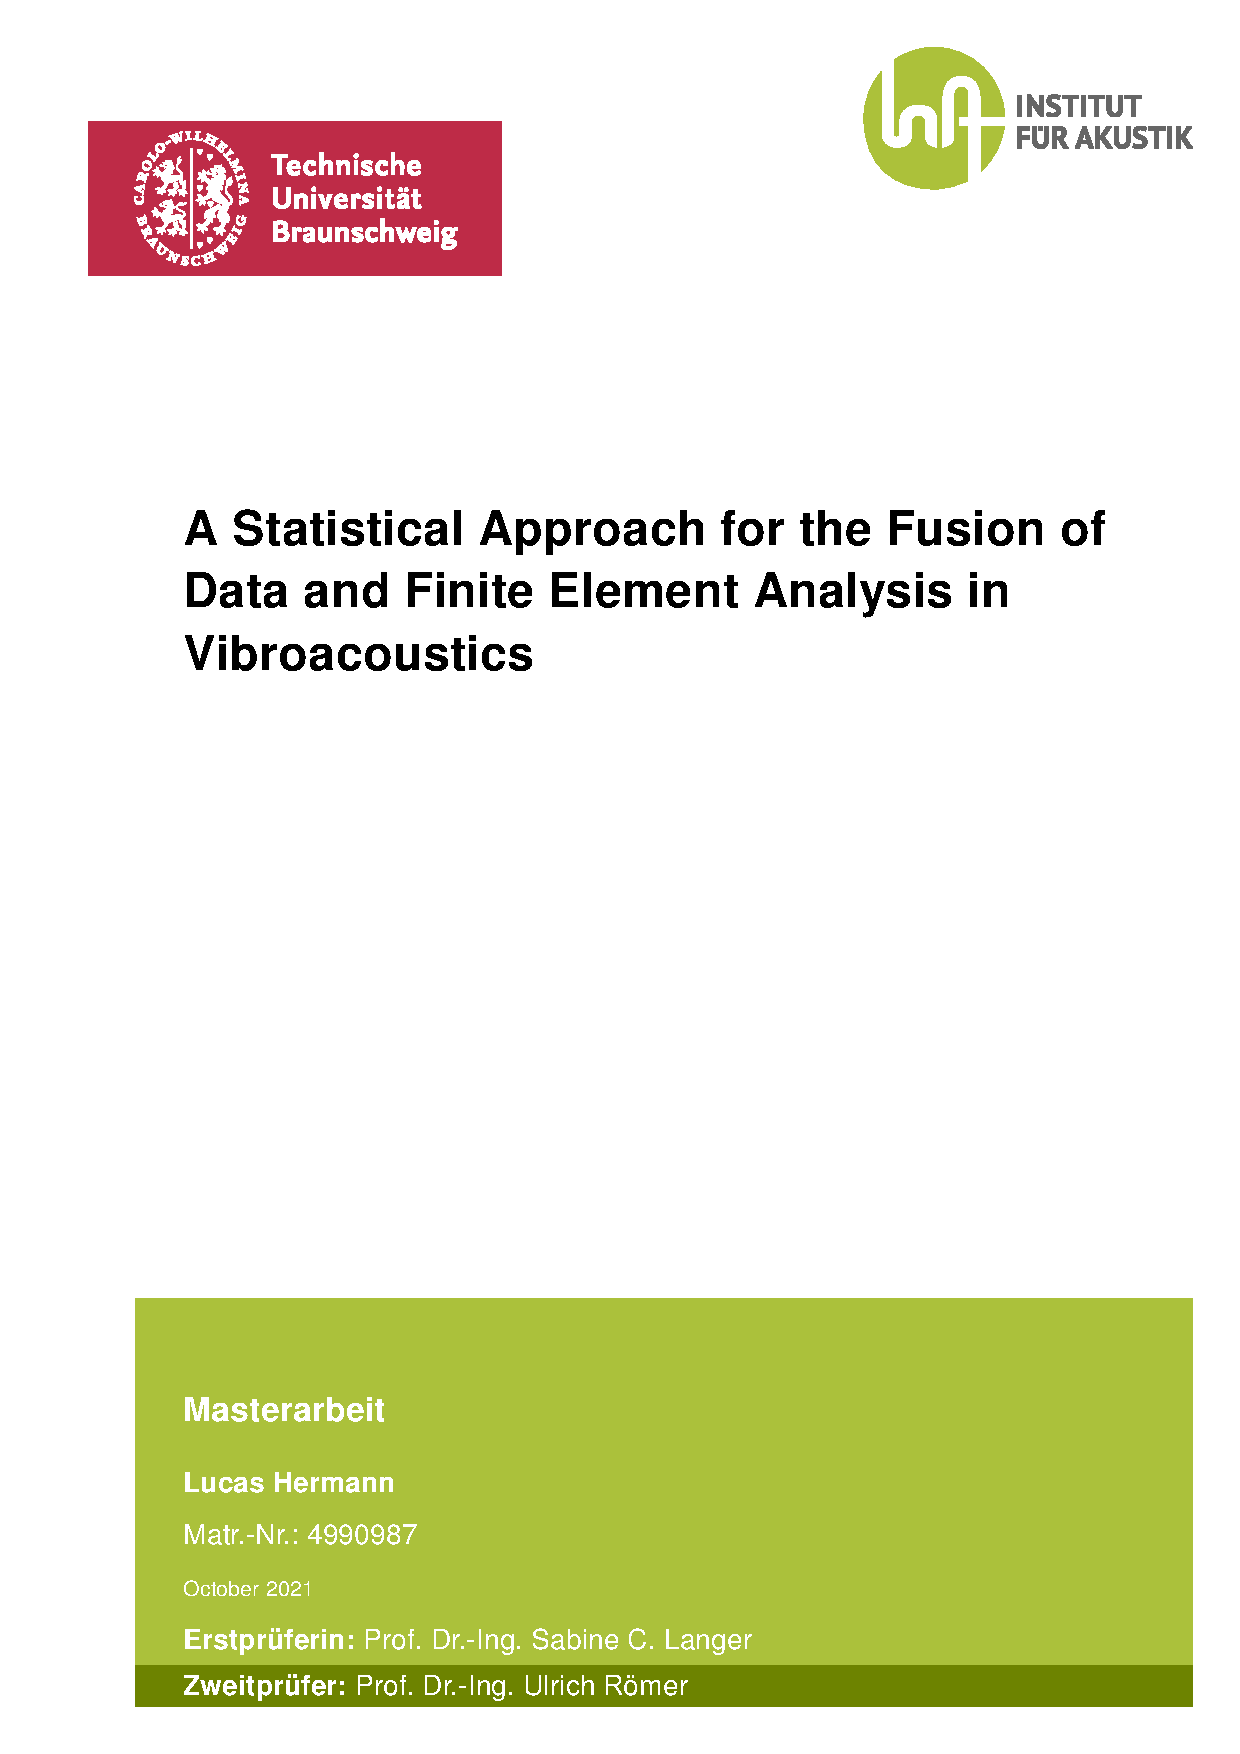
\includepdf[pages=-]{./Deckblatt/2099_StA_Name_Deckblatt.pdf}

\chapter*{Declaration}
Hiermit versichere ich, Lucas Hermann, durch meine Unterschrift, dass ich die
vorliegende Masterarbeit mit dem Titel ``<<Titel>>'' selbständig und ohne Benutzung
anderer als der angegebenen Hilfsmittel angefertigt habe. Alle Stellen, die wörtlich oder sinn-
gemäß aus veröffentlichten oder unveröffentlichten Schriften entnommen sind, habe ich als
solche kenntlich gemacht. Insbesondere sind auch solche Inhalte gekennzeichnet, die von
betreuenden wissenschaftlichen Mitarbeiterinnen und Mitarbeitern des Instituts für Akustik eingebracht wurden.

Die Arbeit oder Auszüge daraus haben noch nicht in gleicher oder ähnlicher Form dieser
oder einer anderen Prüfungsbehörde vorgelegen.

Mir ist bewusst, dass Verstöße gegen die Grundsätze der Selbstständigkeit als Täuschung
betrachtet und entsprechend der Prüfungsordnung geahndet werden.

\begin{flushright}
Braunschweig, \today
\end{flushright}

\vspace{2cm}
\hspace{2cm}\rule{5cm}{1pt}

\hspace{2cm}\small{Lucas Hermann} 

\chapter*{Abstract}
\lipsum[1]

\tableofcontents


\chapter{Introduction}

\textcolor{tubsSecondary}{Dies ist ein Text in \texttt{tubsSecondary}.}
\textcolor{tubsViolet}{Dies ist ein Text in \texttt{tubsViolet}.}
\textcolor{tubsGreenDark}{Dies ist ein Text in \texttt{tubsGreenDark}.}\bigskip

\lipsum[1]

\begin{itemize}
  \item Aufzählungspunkt Eins
  \item Aufzählungspunkt Zwei
    \begin{itemize}
      \item Unter-Aufzählungspunkt Eins
      \item Unter-Aufzählungspunkt Zwei
    \end{itemize}
  \item Aufzählungspunkt Drei
\end{itemize}

\chapter{Theoretical Background}

\section{The Classical Finite Element Method}

\section{Bayesian Inference}
$posterior = \frac{likelihood x prior}{marginal likelihood}$ (Rasmussen p.9)


\section{Gaussian Process Regression}
Gaussian Processes are a class of Bayesian non-parametric models. Non-parametric doesn't mean that there are no parameters involved but rather that there is an infinite number of them. Every realization of a Gaussian process doesn't yield a scalar or vector but a function. One can think of a Gaussian Process as a collection of infinitely many normally distributed random variables, i.e. a generalization of a Gaussian distribution: A vector with infinitely many entries is basically a function. By picking out a finite set of those random variables when discretizing e.g. on an FEM mesh, one obtains a multivariate distribution which is determined by a mean and a covariance matrix. [Rasmussen p.2] Hence, the GP assigns a confidence band to a function where a usual parametric regression wouldn't.

-Regression in general
-differences of a GP regression to e.g. a polynomial regression: every point is assgined an uncertainty

-Herleitung der Kovarianzmatrix, evtl. auch für das standard linear regression modell


\subsection{Prior before observation}

\subsection{Posterior after observation}

\section{The Statistical Finite Element Method}
The differential equation is treated from a Bayesian viewpoint: all parameters are random variables. For dependent parameters not a single distribution but a Gaussian Process is applied. Therefore prior to solving the FEM linear system, the parameter $GP f(x)$ is sampled. That sample is evaluated for each cell in the FEM mesh which makes it necessary to assemble the system matrix with that in mind.

\subsection{Modeling parameters of the PDE}

\subsection{Probabilistic FEM Prior}
The prior before observation is obtained by computing the FEM response $u_h$ of the PDE given all parameters. The random parameters are modeled as GPs. Thereby result a mean $\bar{u_h}$ and a covariance matrix $C_u$. For this being the prior, the GP hyperparameters are chosen deterministically. The covariance matrix is obtained by calculating $C_u = A^{-1} C_{par} A^{-T}$ with $A$ the FEM system matrix and $C_{par}$ the covariance matrix of the respective random parameter's GP. The mean can easily be determined by calculating the deterministic mean of the FEM by using only the GP's mean.
The resulting response $u_h$ is, since it is discretized and not continuous, a multivariate Gaussian distribution.
%
To check convergence of the FEM model, it can be compared to the exact analytically determined system response $u$. 
%
It is assumed that there is a difference between the exact and the calculated FEM response to the true system response. That difference will be reduced by updating the prior with observations.
%
With the basic FEM code set up for a random source term and a deterministic diffusion coefficient, $\bar{u}$ can be obtained by calling
\begin{python}
def get_U_mean(self):
	u_mean = Function(self.V)
	U_mean = u_mean.vector()
	#print(self.mean)
	#print(self.mean[1])
	b_mean = assemble(f_mean*self.v*dx) 
	self.bc.apply(b_mean)
	solstd,A = self.doFEM()  # solstd is unused here.
	solve(A,U_mean,b_mean)
	self.U_mean = U_mean
	return U_mean .
\end{python}
\label{lst:get_u_mean}
$C_u$ can be obtained by calling
\begin{python}
def get_C_u(self):
	C_f = self.get_C_f()
	solstd,A = self.doFEM()
	ident = np.identity(len(self.coordinates))
	self.bc.apply(A)
	A = A.array()
	A_inv = np.linalg.solve(A,ident)
	thresh = 1e-16
	C_u = np.dot( np.dot(A_inv,C_f), np.transpose(A_inv))
	C_u = C_u + 1e-16*(self.sigf**2)*ident
	c_u = np.transpose(self.integratedTestF) * C_u * self.integratedTestF
	return C_u .
\end{python}
\label{lst:get_C_u}
For numerical reasons a small nugget is added to the diagonal of $C_u$. This does not significantly change the result but allows using the Cholesky decomposition.
With $\bar{u}$ and $C_u$ at hand the prior GP is defined as $u \sim \mathcal{GP}(\bar{u},C_u)$. To check if the covariance matrix is correct, a MC approximation $\bar{u}_{MC}$ of the mean can be computed by evaluating the GP $n_{MC}$ times and taking the average. As visible in Figure \ref{fig:u_mean_conv}, the error of $\bar{u}_{MC}$ converges to zero with a slope of 2 on a logarithmic scale. Therefore, $C_u$ indeed has a mean of $\bar{u}$.
The MC samples can be drawn via
\begin{python}
def samplePrior(self):
	U_mean = self.get_U_mean()
	C_u = self.get_C_u()
	priorGP = np.random.multivariate_normal(
		mean = U_mean, cov=C_u,
		size=self.nMC)
	return priorGP
\end{python}

Code for calculating u
direct calculation
MC approximation from GP samples
-error bands

Code for calulating Cu
direct calucaltion
MC approximation
error bands


\begin{figure}[h]
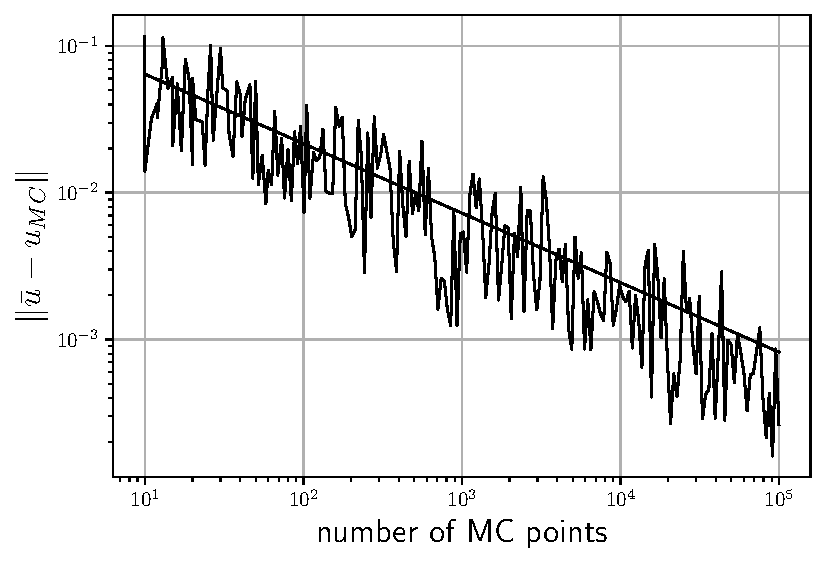
\includegraphics[width=10cm]{pics/MCerrorConv.pdf}
\centering
\caption{Convergence of the error norm for the FEM prior mean}
\end{figure}
\label{fig:u_mean_conv}


\subsection{Modeling Measurement Data}
Measuring data always involves a measurement error: One can never measure any physical quantity without some measurement noise. Therefore, the so-called statistical generating model (Cirak) for a vector of $n_y$ measurements $\bm{y} \in \mathbb{R}^{n_y}$, 
%
\begin{equation}
\bm{y} = \bm{z} + \bm{e} = \rho \bm{P} \bm{u} + \bm{d} + \bm{e} \; ,
\end{equation}
%
consists of response of the true underlying process $\bm{z} \in \mathbb{R}^{n_y}$ at the measurement points and the measurement noise $\bm{e} \in \mathbb{R}^{n_y}$. The true process $\bm{z}$ can further be expressed as a combination of the used model $\bm{u} \in \mathbb{R}^{n_u}$, which tries to describe the true process, and a model discrepancy error $d$ which accounts for the model not being a completely accurate representation of the true physics. The model is scaled using the scaling parameter $\rho \in \mathbb{R}$. It can be evaluated at $n_u$ points which are determined by the FEM mesh but only its evaluations at the measurement points are taken into account by using the projection matrix $\bm{P} \in \mathbb{R}^{n_y \times n_u}$.
%
$e$ is modeled as a multivariate Gaussian 
%
\begin{equation}
\bm{e} \sim p(\bm{e}) = \mathcal{N}(\bm{0}, \bm{C_e})
\end{equation}
with zero mean and the covariance matrix $\bm{C_e} = \sigma_e^2 \bm{I}$ which adds the measurement noise to each entry of $\bm{z}$.
%
The model discrepancy error is, in order to account for a possibly complex behavior, modeled as a GP
\begin{equation}
\bm{d} \sim p(\bm{d} | \sigma_d, l_d) = \mathcal{N}(\bm{0},\bm{C_d})
\end{equation}
which $\sigma_d, l_d$ the unknown parameters of a squared exponential kernel function. Evaluating it at the measurement positions, the GP is represented by a multivariate Gaussian with a covariance matrix $\bm{C_d} \in \mathbb{R}^{n_y \times n_y}$.

The projection matrix $P$ is constructed by evaluating all FEM ansatz functions of the mesh at the $n_y$ measurement positions. The result is a sparse matrix with most entries zero and only those entries non zero that correspond to the ansatz functions $\Phi_i(\bm{\bm{x}})$ associated with the finite element in which the measurement positions lie.
This computation for linear ansatz functions can easily be implemented in Python using Fenics:

\begin{python}
def getP(self,y_points):
	ny = len(y_points)
	P = np.zeros((ny, self.ne+1), dtype = float) #with ne the number of elements
	for j,point in enumerate(y_points):
		x = np.array([point])
		x_point = Point(x)
		bbt = self.mesh.bounding_box_tree()
		cell_id = bbt.compute_first_entity_collision(x_point)
		cell = Cell(self.mesh, cell_id)
		coordinate_dofs = cell.get_vertex_coordinates()
		values = np.ones(1, dtype=float)
		for i in range(self.el.space_dimension()): 
			phi_x = self.el.evaluate_basis(np.array(i),x 
				,np.array(coordinate_dofs),cell.orientation())
			P[j,cell_id+i] = phi_x
	self.Pu = np.dot(P,self.U_mean)
	return P
\end{python}
\label{lst:getP}



\subsection{Estimation of Hyperparameters}
Below it was already stated that the hyperparameters for computing the model discrepancy covariance matrix $\bm{C_d}$ are not known. The scaling factor $\rho$ is not known, as well. The measurement data can be used to estimate these parameters, collected in the hyperparameter vector $\bm{w}$, with Bayes' rule 
%
\begin{equation}
p(w|y) = \frac{P(y|w) p(w)}{\int P(y|w) p(w) dw}
\end{equation}
%
where the denominator, which only serves as a normalization constant, can be dropped if only a point estimate of the hyperparameters is needed. This approach is indeed non-bayesian because no probability density of the hyperparameters is computed. For multiple measurements $y_i$ with a total number of $n_o$ there holds 
\begin{equation}
P(Y|w) = \prod_{i=1}^{n_o} p(\bm{y_i}) \; 
\end{equation}
which replaces $P(y|w)$.
If no prior knowledge of the parameters is available, it is possible to use an uninformative prior $p(w) = 1$.
The equation then basically states that $p(w|Y) \propto P(Y|w)$ which means that maximizing  $P(Y|w)$, i.e. the likelihood to measure $Y$ given a set of hyperparameters, yields the optimal vector of hyperparameters for the given data. 
The marginal likelihood $P(y|w)$, marginal because ?!?!?!, can be expressed as 
\begin{equation}
p(y|w) = \mathcal{N}(\rho \bm{P}\bar{u}, \bm{C_d}+\bm{C_e} + \rho^2 \bm{P} \bm{C_u} \bm{P}^T)
\end{equation}
because, as stated above, all components of the statistical generating model are Gaussian.
The equation for the corresponding PDF reads
\begin{equation}
p(y|w) = \frac{1}{(2 \pi)^{n/2} |K|^{1/2} } \exp \left(   -\frac{1}{2} (y - \rho \bm{P}\bar{u})^T \bm{K}^{-1} (y - \rho \bm{P}\bar{u})   \right)
\end{equation}
with
\begin{equation}
K = \bm{C_d}+\bm{C_e} + \rho^2 \bm{P} \bm{C_u} \bm{P}^T \; .
\end{equation}
%
To make further calculations easier the exponential function can be removed by taking the negative $\log$ of the function (Rasmussen):
\begin{equation}
- \log p(y|w) = \frac{n}{2} \log(2 \pi) + \frac{1}{2} \log |\bm{K}| + \frac{1}{2}(\rho \bm{P}\bar{u} - y)^T \bm{K}^{-1} (\rho \bm{P}\bar{u} - y) 
\label{eqn:neglog}
\end{equation}
This also improves numerical stability because products of possibly very small factors can become smaller than machine accuracy. The log replaces products with sums.
Because of taking the negative $\log$, (\ref{eqn:neglog}) now needs to be minimized instead of maximized. 

\paragraph{Cholesky Decompositon}
[Gentle 1998 p.93-95]
For numerical stability reasons $\bm{K}^{-1}$ should not be calculated directly. Instead, the linear system is solved. Additionally, if $K$ is symmetric and positive-semidefinite, computing the lower triangular matrix using the Cholesky decomposition 
\begin{equation}
K = LL^T
\end{equation}
makes the calculation quicker and yields the also needed determinant of $K$ as a by-product. 
A generic linear system is defined as $A x = b$. It is solved for $x$, so the inverse of $A$ is needed. In this case for (\ref{eqn:neglog}) there holds $A=K$ and $b = y$, since the inverse of $K$ is meant to be found. Defining $x = K^{-1}y$ there holds
\begin{equation}
K \times K^{-1} \times y = y
\end{equation}
%
With $L$ the lower triangular matrix of $K$ obtained by 
\begin{lstlisting}[language=Python]
L = scipy.linalg.cho_factor(K)
\end{lstlisting}
the linear system can now be solved for $x = K^{-1}y$ with
\begin{lstlisting}[language=Python]
K_inv_y = scipy.linalg.cho_solve(L, y) .
\end{lstlisting}

The determinant of any triangular matrix is defined as the product of its diagonal entries [http://www.math.lsa.umich.edu/~hochster/419/det.html]. Therefore the lower triangular matrix $L$ can be used to efficiently calculate the determinant of $K$. There holds
\begin{equation}
det K = det L det L^T = det L ^2
\end{equation}
and therefore
\begin{equation}
det K = \left(    \prod_{i=1}^{n_y}  L_{i,i}  \right)^2
\label{eqn:CholDet}
\end{equation}

Since in (\ref{eqn:neglog}) the $\log$ likelihood is used, (\ref{eqn:CholDet}) can be simplified to a sum:

\begin{align*}
\log{det K} &= \log{det L}^2 \\
&= 2 \sum_{i=0}^{n_y} \log{L_{i,i}}
\end{align*}

\subsubsection{Minimization of the Negative log-Likelihood}
The best possible set of hyperparameters $\bm{w}$ for (\ref{eqn:neglog}) to be as small as possible has to be found. That can be achieved by using a gradient based optimizer or by sampling the parameter space with, e.g., a MCMC approach.
\paragraph{MCMC}
Markov Chain Monte Carlo (MCMC) is a very efficient sampling method. Just as standard MC, it can be used to draw samples from a given distribution. The advantage of MCMC is now that an algorithm finds a relatively small set of samples which is able to describe the distribution very accurately. The result is a distribution for the hyperparameters of which e.g. the mean can be deduced. One common algorithm is the metropolis algorithm.
The metropolis algorithm is a special case of MCMC for a symmetric proposal distribution.
Metropolis algorithm as code. 



\paragraph{L-BGFS}
L-BGFS is a gradient based optimizer. It doesn't deliver a distribution for the hyperparameters but only a point estimate.
For the optimization with L-BGFS the derivative of (\ref{eqn:neglog}) is needed. It can be computed as follows.


\subsection{Inference of the Posterior Density}
To infer the posterior density, observed data is necessary. These can be obtained by either actually measuring a physical process or by generating synthetic data which allows developing and improving the statFEM model already before having to set up an experiment and take real measurements beforehand.
%
Sampling from a synthetic source or from the real physical response yields the observation vector
%
\begin{equation}
\bm{y} = {z} + {e}
\end{equation}
%
with $z$ the real response and $e$ the measurement error which is also a part of $\bm{y}$ for the synthetic observations. It can be seen that the model mismatch error $\bm{d}$ is, as opposed to eq. (), not part of the equation because it is only part of the FEM modeling error. 
%
The data is observed on multiple measurement  points $n_y$ throughout the domain. It can be chosen if the data is assumed to be deterministic or to be random. For the deterministic case only one value is measured for each measurement point. In the random case many measurements are taken per point what leads to a probability distribution for each point.
%
Now, Bayes' rule can be applied to update the prior with the observations.
The result of this operation is
%
\begin{equation}
p(u|y) = \mathcal{N}(\bar{u_{|y}}, C_{u|y})
\end{equation}
%
with
%
\begin{equation}
\bar{u_{|y}} = C_{u|y} \left(   \rho P^T  (C_d + C_e)^{-1}  y  +  C_u^{-1}  \bar{u}   \right)
\end{equation}
and
\begin{equation}
C_{u|y} = \left(      \rho^2  P^T   (C_d + C_e)^{-1}  P  +  C_u^{-1}    \right)^{-1}
\end{equation}





\chapter{1D Example and Application in Vibroacoustics}

\section{Simple 1D example}
\paragraph{Choice of PDE}
The Poisson equation 
%%
\begin{equation}
- \nabla \cdot \mu(x) \nabla u(x) = f(x)
\label{eqn:Poisson}
\end{equation}
%%
is chosen as the governing equation. It is an elliptic partial differential equation (PDE). In this work it is used as a simple 1D example to illustrate how the statistical FEM and especially the Gaussian Process Regression works.
The most standard form of it does not, contrary to this example, include $\mu(x) \in \mathbb{R}^+$ which is the diffusion coefficient dependent on the spatial variable $x$. The right-hand side consists of the source term $f(x)\in \mathbb{R}$. Both $\mu (x)$ and $f(x)$ are the free parameters in this case. The equation is solved for the unknown  $u(x)$ in the domain $\Omega = (0,1)$ with the boundary condition $u(x) = 0$ on $x=0$ and $x=1$.
%
For a first example there holds $\mu(x)=1$. $f(x)$ is modeled as a Gaussian Process [Cirak]
%
\begin{equation}
f(\bm{x}) \sim \mathcal{GP} \left( \bar{f}(\bm{x}), c_f(\bm{x},\bm{x}')\right) \;.
\end{equation}
%
\paragraph{Construction of the GP}
The mean function of the GP is set to $\bar{f}(x) = 1.0$. For the covariance function at first a squared exponential kernel 
%
\begin{equation}
c_f(\bm{x},\bm{x}') =    \sigma_{f}^2 \exp \left(-  \frac{\left \| \bm{x}-{\bm{x}}' \right \|^2}{2l_{f}^2} \right )       
\label{eqn:sqEx_f}
\end{equation}
%
is used with the standard deviation $\sigma_{f} = 0.1$ and the length scale $l_{f} = 0.4$.
In Python the kernel is directly implemented as a function which takes two lists and the parameters as input variables [Murphy]:
\begin{lstlisting}[language=Python]
def squared_exponential(xa, xb, lf, sigf):
    sq_norm = -0.5 * scipy.spatial.distance.cdist(xa, xb, 'sqeuclidean') \
    	* (1/lf**2)
    return sigf**2 * np.exp(sq_norm) .
\end{lstlisting}
\label{lst:sqEx}
%
Here, the parameters are fixed but in a later example a method on how to infer the optimum position for these will be studied.

Having prepared the mean function and the kernel, which can be considered the prior in a GP regression setting, a sample of the GP can be drawn. For this points have to be chosen on which the kernel is evaluated. These are the test points and, according to [Cirak], correspond to the center of the FEM cells. This implies that there are as many test points as FEM cells and therefore the coordinates of the FEM mesh can directly be used to compute the covariance matrix. For that (\ref{eqn:sqEx_f}) is evaluated at $\bm{x} = \bm{x}'$ with $\bm{x}$ the vector of test points. 

A GP has the marginalization property: if you sample it at a finite number of points it yields a multivariate Gaussian distribution $\mathcal{N}(\bar{\bm{f}},\bm{C_f})$ with $\bar{\bm{f}}$ the mean vector and $\bm{C_f}$ the covariance matrix while still describing the underlying continuous sample.
According to [Rasmussen] sampling from a multivariate Gaussian distribution works as follows: To obtain $n$ samples from the prior, at first $n$ samples of a standard normal distribution, also called Gaussian white noise, $e \sim \mathcal{N}(0,1)$ have to be drawn. Computing the Cholesky decomposition of the covariance matrix $\bm{C_f} = LL^T$, which can also be thought of as taking the square root of a matrix, yields the lower triangular matrix $L$. Samples can now easily be drawn from $\bm{f} = \bar{\bm{f}} + Le$ which is a multivariate Gaussian distribution with a mean $\bm{f}$ and a covariance $\bm{C_f}$.

Sample: Normal distribution times std dev. GP with n points is basically a multivariate gaussian with n dimensions. therefore we need the std dev. for a univariate gaussian thats . 

For the observations made in a later step it is assumed that there is some measurement noise. This is modeled as an added variance $\sigma_{n}^2$ on the diagonal of the prior covariance matrix. An additional effect of this added noise is the improved numerical stability of the covariance matrix which is important for computing the Cholesky decomposition.

\section{1D Vibroacoustics Example}
Helmholtz Equation. Looks similar to the Poisson equation but the right side differs. It's the eigenvalue problem for the laplace operator.

\lipsum[2-5] %\cite{campolina}



\chapter{Results and Discussion}

\lipsum[1-3] %\cite{Langer2019}

\section{Section 1}

\lipsum[4-7] %\cite{Yaghoubi:2017}


\begin{thebibliography}{4}
%
\bibitem{campolina}
Campolina, B.: Vibroacoustic modelling of aircraft double-walls with structural links using Statistical
Energy Analysis (SEA). Acoustics [physics.class-ph]. Université de Sherbrooke; Université Pierre
et Marie Curie - Paris VI (2012)

\bibitem{Langer2019}
Langer, S.C., Blech, C.: Cabin noise prediction using wave‐resolving aircraft models. Proc. Appl. Math. Mech., Vol. 12 (1) (2019): e201900388. doi:10.1002/pamm.201900388

\bibitem {Yaghoubi:2017} Yaghoubi, V., Marelli, S., Sudret, B., Abrahamsson, T.: Sparse polynomial chaos expansions of frequency response functions using stochastic frequency transformation, Probabilistic Engineering Mechanics, volume 48, pages 39-58 (2017)
\end{thebibliography}

\end{document}
